\chapter{Introduction}
\label{cha:introduction}

[Intro]

The work described in this thesis is part of a larger project that aims to develop a system ... 
The project is divided into three main parts: data analysis, machine learning, and cloud infrastructure as shown in Figure \ref{fig:project_parts}.

\begin{figure}[htb]
    \centering
    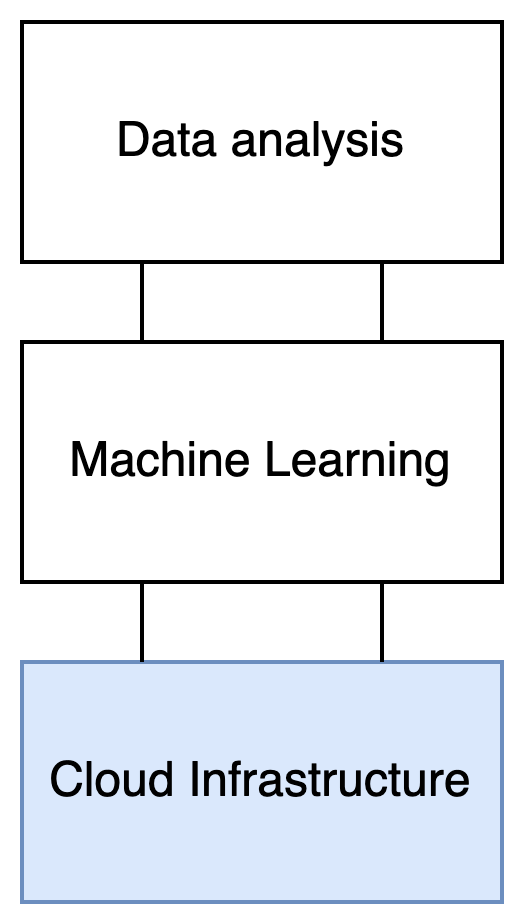
\includegraphics[width=0.25\linewidth]{images/project_parts.png}
    \caption{Project parts}
    \label{fig:project_parts}
\end{figure}

\section{Context}
\label{sec:context}

Computational sustainability

GreenOps

GreenOps for FinOps
(Operating for GreenOps may lead to reduced costs)

\subsection{GreenOps}
\subsection{Geographical shifting and Time shifting}
\subsection{Carbon-aware workload scheduling}


Cloud sustainability

Current Sustainable Cloud Computing Landscape
we are in the infrastructure tooling section
in particular scheduling (day 1 operatsion

scaling and resource tuning are usuaully day 2 operation

the system was envisioned with this in mind and is capable of doing that

\section{Problem statement}
\label{sec:problem}

test


Use cases (basic ones for the beginning) higher level explanation here
first use case ("GreenOps" VM scheduling)

second: scaling down a vm 
infrastructure already put in place

the system was designed with flexibility in mind therefore a workload could be potentially anything
the condition is just to be represented in some way and have something else do certain actions based on that representation
As we will see in section XXX, the most simple of this would be K8s operators
this is described in section XYZ

\section{Method}

Developing a real solution, integrating it on top of OSS

production-ready solution

we are on the consumer side, not on the provider side

System architecture to start with: Saima's + Krateo platform

integration into an existing platform (krateo)


leveraging krateo componenets

Krateo Core Provider and cdc instead of developing 1 or more K8s operators from scratch


analysis of possible solutions
implemnted poc 

Initial analysis of a solution with operators were tried

A PoC comprising 1 operator was created 
``Synchronization operation"
cons: maintainer costs



ideation and creation of architectural diagrams



tackling first use case
but create a system that is flexible enough to be used for other use cases as well

\section{Personal contribution}

The project, ideated and supervisioned by Prof. Fiore is mainly divided into 3 parts.

exploratory data analysis
data preparation

model training
model selection

infrastructure part

GOAL
The goal of the project is to employ mainly time-shifting and geographical shifting for the scheduling of workload leveraging a multi-cloud setting.
We can choose to schedule workloads in periods and regions with low carbon intensity (when renewables are plentiful). 
Therefore, targeted workloads are the ones that are not time-sensitive but instead are quite delay-tolerant. For example training a machine learning model could wait until a period of low carbon intensity. Another example is shifting video / image processing, as Google is doing.
Kubernetes is leveraged as a platform for scheduling and managing workloads on different cloud providers.
Long term goal: “Using electricity when the carbon intensity is low is the best way to ensure investment flows towards low-carbon emitting plants and away from high-carbon emitting plants”.

\newpage
